\section{Introduction}
\label{sec:intro}

LLM-based agents~\cite{achiam2023gpt4,openclaw,opencode,claudecode,openai-codex-cli,wang2024agentsurvey} are reshaping how software tasks get done.
Instead of writing code by hand, a developer describes a goal,
and the agent reasons, invokes tools, and delivers the result~\cite{yao2023react,qin2023toolllm}.
To support this paradigm, a growing ecosystem of \emph{skills}~\cite{claude-agent-skills,anthropic-skills-repo,openclaw-medical-skills,skillssh} has emerged
to make agent execution more reliable and practical.
Skills primarily consist of natural language descriptions and scripts, encapsulating domain-specific
procedures and best practices~\cite{anthropic-skills-blog}.
Over 100,000 skills are now distributed across major platforms~\cite{clawhub, skillssh},
spanning data analysis, finance, office automation, programming,
and beyond.

However, current agents' support for skills is simplistic: skills are treated as
additional context and passed directly to the model. Models differ substantially in
their ability to understand and execute skills~\cite{lu2024agentbench, han2026swe, li2026skillsbench}.
Across eight models spanning a range of scales,
enabling skills degrades performance on 15\% of tasks overall (e.g., 7\% for Opus 4.6 and 25\% for Qwen3-30B).
For another 17\% of tasks, scores remain unchanged (excluding tasks with 100\% completion),
and on up to 87\% of tasks, at least one model shows no improvement after skill usage.
Recent work~\cite{han2026swe} has reached similar conclusions, finding that on the SWE-Benchmark, 39 out of 49 skills showed no score improvement, and 3 skills experienced significant score degradation.

\begin{figure}[t]
  \centering
  \setlength{\abovecaptionskip}{5pt}
  \setlength{\belowcaptionskip}{-10pt}
  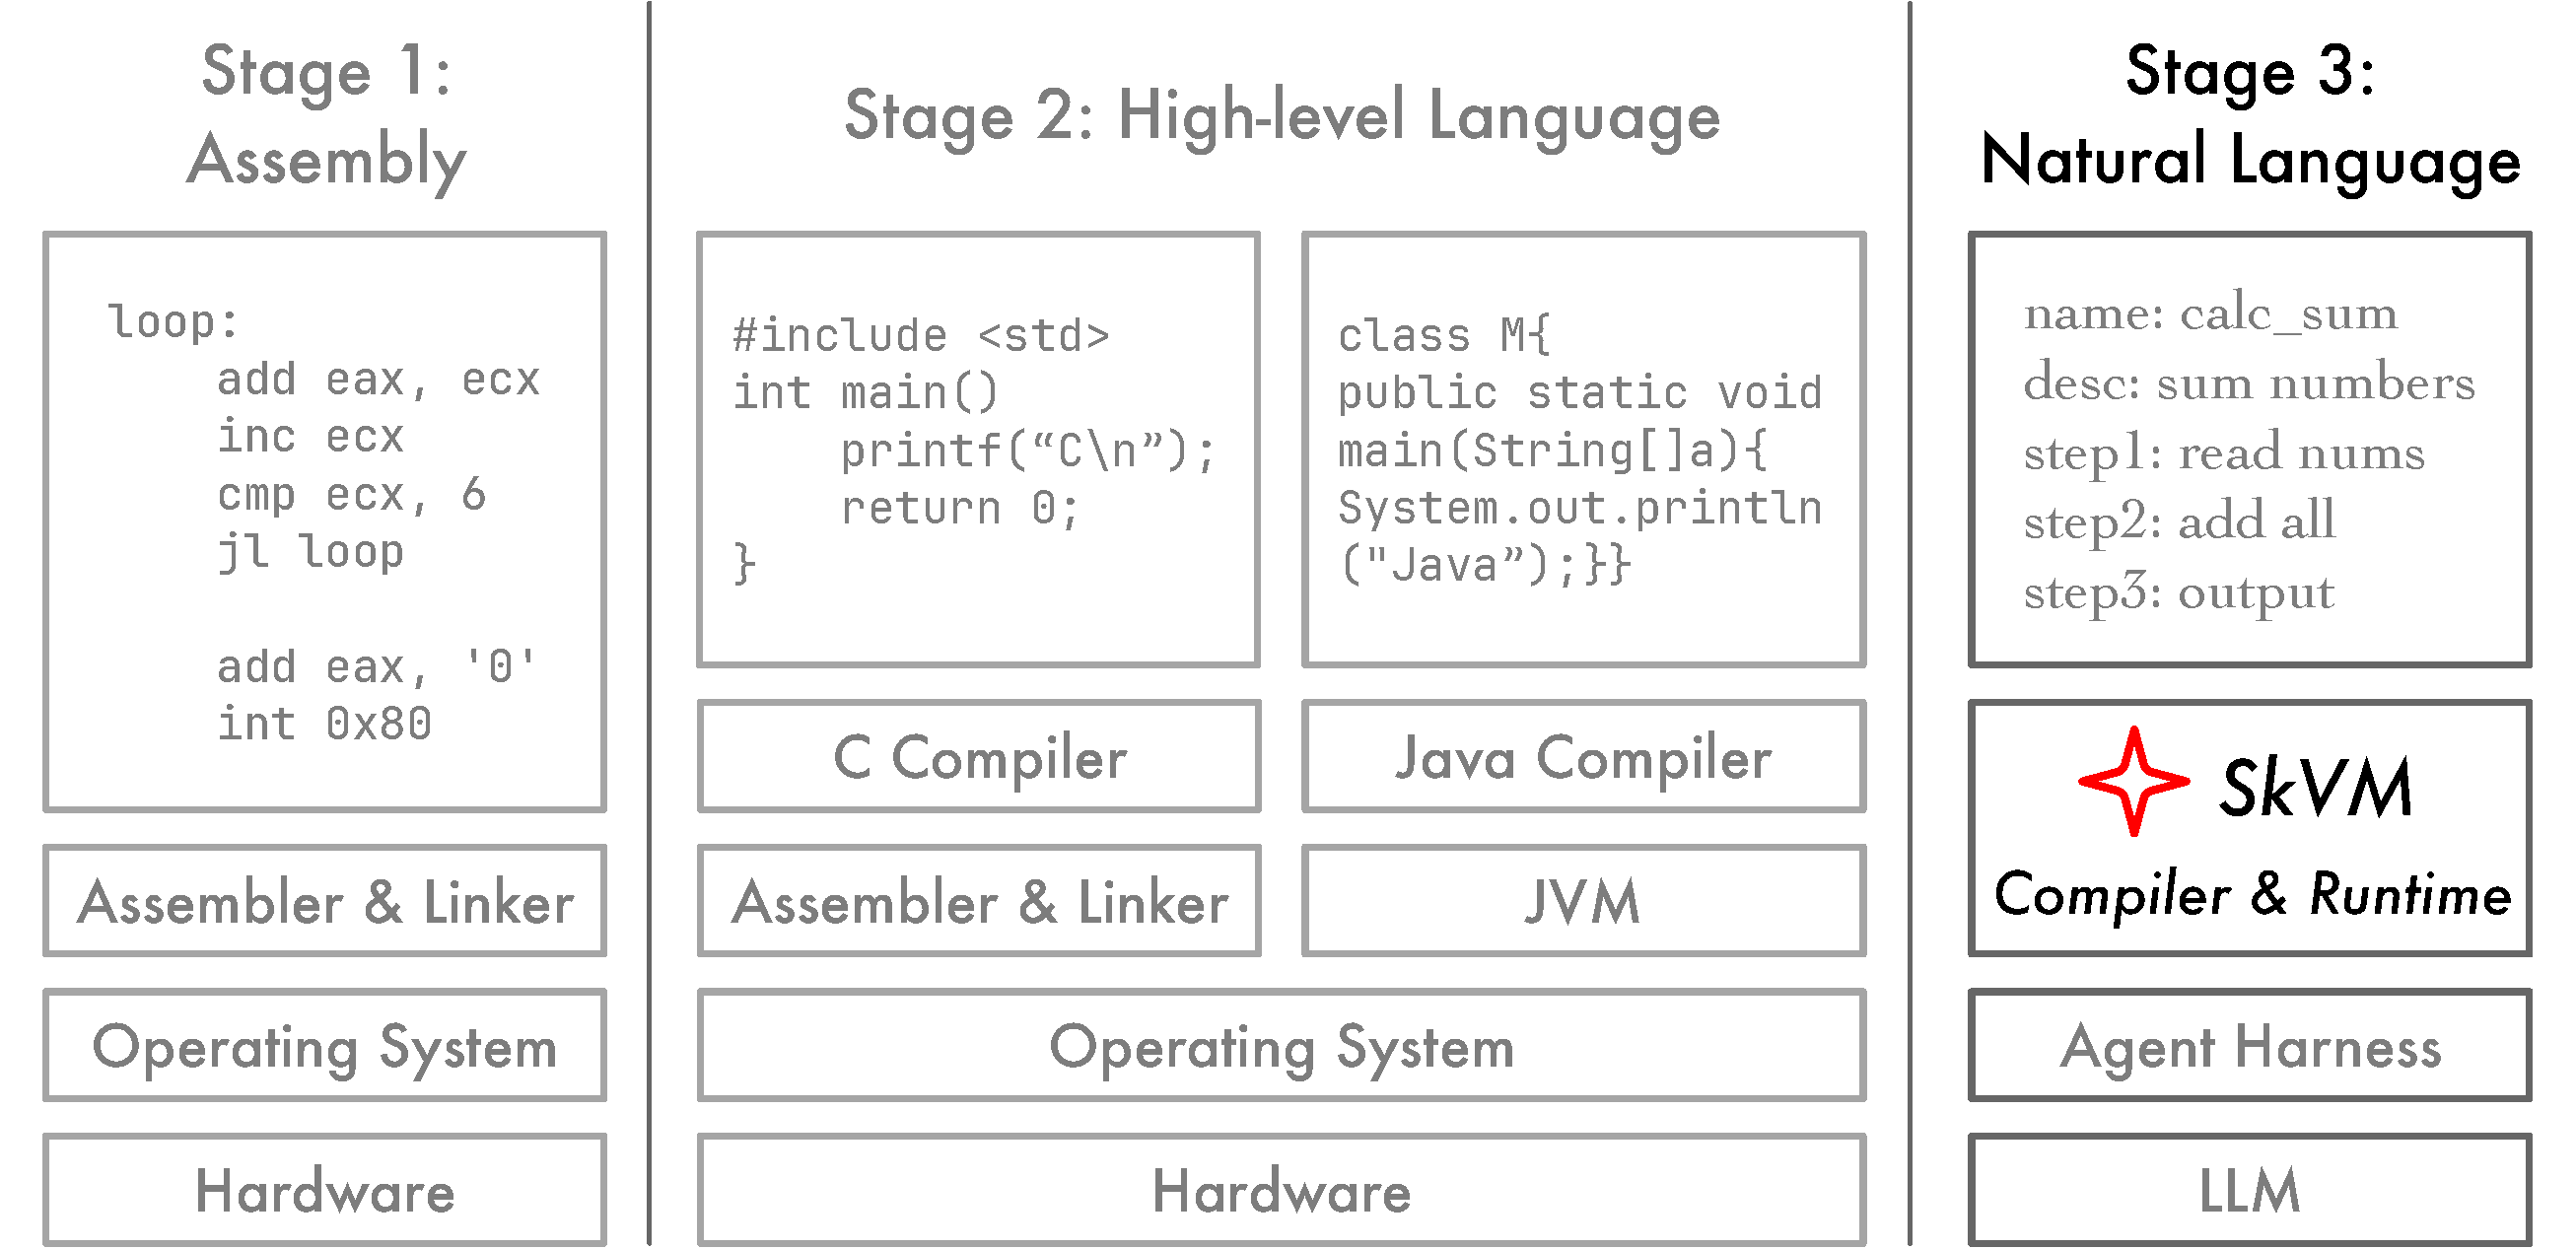
\includegraphics[width=\columnwidth]{figures/skillos_arch.pdf}
  \caption{Evolution of programming abstractions. Skills are
    the current frontier: natural language programs of hundreds of lines
    that lack a compiler and runtime for cross-target portability.}
  \label{fig:evolution}
\end{figure}

We attribute these issues to two factors: (1) even when a skill is loaded, the model may ignore its guidance during execution;
and (2) even when the model follows the skill, the skill's assumptions about model capabilities may not match the model's actual competence.
Beyond differences in task completion gains, the semi-structured code snippets and workflow-style formats
common in current skills also incur substantial token overhead (e.g., 451\% token increase while pass rates remain unchanged~\cite{han2026swe}) and higher latency during execution.

This problem arises from a fundamental mismatch between static skills and the variability of underlying models and agent harnesses.
The capabilities a skill demands may not align with the capabilities
of the LLM invoked at runtime. Revisiting the evolution of computing paradigms~\cite{stroustrup2013c++, venners1998java, cramer1997compiling} (as shown in Figure~\ref{fig:evolution}), we observe that
in the agent era, \textbf{skills are code}, and \textbf{LLMs are processors}. Yet today, no mechanism
exists to efficiently and reliably execute skills across heterogeneous LLMs and agent harnesses.


Inspired by how classical computing systems handle code, we introduce
\sys, a compilation and runtime system for skills that enables
efficient cross-model execution and provides unified underlying
support for skill execution. Through \sys, skills are compiled
into forms tailored to different models, allowing each model to
better understand and execute skills. Furthermore, \sys provides a unified runtime
environment that systematically manages skill loading, parsing,
and concurrent execution.

\textit{We structure \sys around classical compilation techniques:
interpreted execution~\cite{jansen2007interpretation}, ahead-of-time (AOT) compilation~\cite{serrano2021javascript, serrano2018javascript}, and just-in-time (JIT)
optimization~\cite{aho2006compilers, aycock2003jit, suganuma2000overview, ishizaki2000study, cramer1997compiling}.} Currently, agents handle skills using only interpreted
execution, feeding raw skill text directly to the model. This approach
hampers skill portability and execution efficiency. In contrast, \sys further applies
AOT and JIT compilation to optimize for diverse backend models and execution
environments:

\textbf{AOT compilation:} Skills inherently encode requirements of model capabilities, environment configuration, and parallelism opportunities. 
Therefore, \sys analyzes these requirements before execution and optimizes skills accordingly.
\emph{Capability-based compilation} characterizes the capability gap between LLMs and skill requirements by extracting 26 primitive capabilities. 
Each capability abstracts a distinct dimension of model behavior with multiple proficiency levels.
The compiler measures the target model against these capability dimensions and adapts the skill specification to better align with model strengths and limitations.
Second, \emph{environment binding} extracts implicit dependencies on packages and tools from skill descriptions and generates setup scripts executable at load time, ensuring all dependencies are satisfied before skill execution.
Finally, \emph{concurrency extraction} draws inspiration from classical compiler optimizations for data-level parallelism (DLP)~\cite{kalathingal2016dynamic}, instruction-level parallelism (ILP)~\cite{ranganathan1998empirical, kastner2001ilp}, and thread-level parallelism (TLP)~\cite{redstone2003mini}. It extracts parallelism opportunities at similar three granularities from skills and explicitly exposes them to the agent harness, thereby improving task execution efficiency.


\textbf{JIT optimization:} At runtime, \sys leverages runtime information to continuously optimize skill performance and correctness. 
\emph{Code solidification:} Skills may contain parameterized script templates which may be instantiated multiple times during different executions. 
JIT compilation materializes these high-frequency templates into instantiated executable code, bypassing LLM parsing. 
\emph{Adaptive recompilation:} JIT monitoring tracks model execution and adaptively recompiles skills when
capability gaps emerge, ensuring skills can self-improve through iterative optimization.

After skill compilation completes, the skill runtime parses compiled skill artifacts (including optimized
skills, instantiated scripts, and concurrency dependency graphs) rather than
simply passing raw text to the model. Additionally, the skill
runtime coordinates with the system's available resources and tool capabilities
to schedule agent execution in real time, and ensures stable and reliable agent execution.

We evaluate \sys across eight LLMs of varying scales and three agent harnesses, covering SkillsBench~\cite{li2026skillsbench} and representative skill tasks (118 tasks).
Results demonstrate that \sys significantly improves task completion rates (averaging 15.3\%) across different models and agent harnesses~\cite{claudecode,opencode}.
Furthermore, for tasks that can be completed, \sys reduces token consumption up to 40\%.
In terms of performance, \sys achieves 3.2$\times$--50$\times$ wall-clock speedups through fine-grained parallelization and JIT code solidification.
